\chapter{Introduction}
\label{chapter:intro}
\graphicspath{{./chapters/c1_intro/figures/}}
%=========== MAIN ================
Single-molecule technique invented in the 1990s has quickly developed into a research field by itself. It has revolutionized the field of molecular biology, imaging (super-resolution), catalysis to name a few. In this thesis, we will push the single-molecule studies to light absorbers with low quantum yield and to high concentration of probe molecules through fluorescence enhancement by gold nanorods. Following single-molecule trajectories, we will explore variations in the electron transfer rates of ``azurin'' both spatially and dynamically. The evidences for conformational substates will be discussed based on dynamic heterogeneities. In this chapter we have tried to cover basic principles required to get a reasonable understanding of the rest of the content of the thesis.  


\section{Fluorescence}
The absorption and subsequent emission of light by materials is called fluorescence.
The term Fluorescence was named by \textit{George Gabriel Stokes} after observing ultraviolet light being transformed into visible light in the mineral fluorite.\cite{Stokes1852}
A molecule is excited to a higher electronic energy state after absorbing a resonant photon.
Each electronic energy level is associated with vibrational and rotational energy levels.
The excess vibrational energy gained in the excited state is quickly lost to the surrounding in a time period of sub-picoseconds and the molecule stays in its zero vibrational level of excited state for about nanoseconds.
If it is allowed to come down to the ground state which is decided by the spin states (singlet allowed) of the paired electrons and Franck-Condon principle, \textit{fluorescence emission} is observed.
The emitted photon has a smaller energy than the absorbed photon which is known as Stoke's shift and the total time it takes to come down to the ground state is called fluorescence lifetime typically \SI{10}{\ns}.
If the system crosses over from singlet excited to the triplet state, emission may be observed at even longer wavelength and even longer lifetime which is known as \textit{phosphorescence}.
The processes between the absorption and emission are normally represented graphically by Jablonski diagram.\cite{RohatgiMukherjee1979k,Lakowicz1999book}

\begin{figure}
	\centering
	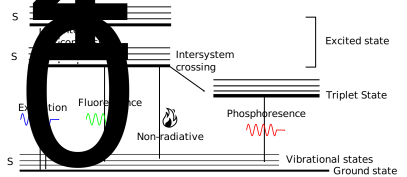
\includegraphics[width=0.8\textwidth]{jablonski}
	\caption{\textbf{Jablonski Diagram.} Simplified model of transitions in fluorescence. A molecule is promoted to the excited electronic state by absorbing a photon. Non-radiative relaxation processes bring it to the lowest vibrational state of first electronic state from where it can either emit a photon or release the energy as heat or make a transition to the triplet state.}
	\label{fig:jablonski}
\end{figure}

Natural materials that show fluorescence include minerals, tissue in plants and animals.
Among biological molecules nicotinamide adenine dinucleotide (NADH), flavins (FAD), chlorophyll are abundantly found fluorescing.\cite{blacker2014separating,siano1989nadh,genty1989the}
Extrinsic fluorophores are also synthesized with high quantum yield and varying color which include synthetic dyes, quantum dots.\cite{atkinson1952the,alivisatos1996semiconductor}
Fluorescence has a huge advantage of very low background which enables their detection with very low concentration of fluorescent molecules.
This was very important for biological imaging as little quantity of such markers keep the system under study unaffected.\cite{white1987an}
Not only external fluorophores can be used for biological marking, the cells can also be gene-edited to produce their own fluorophores called fluorescent protein (GFP).\cite{tsien1998the,chalfie1994green}
Now a days it is unthinkable to use a biology or analytical chemistry lab without fluorescence technique.

\section{Single Molecule Spectroscopy}
The thought experiment by Jean Perrin to observe single fluorescent molecules was materialized for the first time in 1990s at an extremely low temperature and in an advanced laboratory.\cite{orrit1990single}
The rapid development of optical microscope, lasers, dyes and detectors now made it possible to detect single molecules at room temperature even on a bench top.\cite{xie1998optical,weiss1999fluorescence,moerner1999illuminating}
Not only it has grown itself into an important research field, the concept is now heavily used in molecular biology, super-resolution microscopy, quantum computing, catalysis to name a few.\cite{zhuang2000a,huang2008threedimensional,eisaman2011invited,lounis2005singlephoton,roeffaers2007singlemolecule}
The following advantages provided by single-molecule study make it an indispensable technique:
\begin{itemize}
	\item \textbf{No averaging.} Ensemble measurements provide mean value of a physical quantity, looking at average behavior of vast number of molecules.
	In complex medium like in condensed matters and cellular matrix, each molecule is in a different microscopic surrounding experiencing different forces and resistances.
	Single molecule measurements provide distribution of quantities distinguishing the subpopulations within the system with distinct characteristics.
	For example different host molecules even in a crystalline (ordered structure) solids show different spectral lines and line widths discovering the imperfections.\cite{kozankiewicz1994single,reilly1993spectral}
	Small domains of \SIrange{50}{700}{\nm} in a cell membrane are located based on the difference in the diffusion coefficient of single molecules in the membrane.\cite{lommerse2004singlemolecule}
	Rare species that are lost in ensemble measurements can be identified and investigated in SM studies.
	The distribution in spatial dimension is called static heterogeneity.
	\item \textbf{Time dependent fluctuation.} Dynamics of systems can be studied without the need for synchronization (kinetic measurements in ensemble often require synchronization).
	Single molecule measurements at equilibrium provide direct access to both dynamics and statistics of molecular complexes.
	They also provide information on a wide range of time scale from microseconds to tens of seconds extracting translational, orientational, enzymatic-turnovers and protein folding-unfolding events.\cite{schmidt1996imaging,ruiter1997single,lu1998single-molecule,schuler2002probing}
	the distribution along a time trajectory is called dynamic heterogeneity.
	\item \textbf{Local reporter} As single molecule detection is based on optical microscopy, the observer can be far away from the molecule itself provided the intervening medium is optically transparent.
	The trajectory of the reporter molecules deep inside the cell can be tracked without physical intervention to follow the activities of the host.
	\item \textbf{Tool.} Single-molecules are finding their ways to be used as tools to perform different tasks.
	As the transitions in the excitation of single-molecules are quantum in nature, they can be used as source of pure single photons for quantum computing.\cite{lounis2000single,lounis2005singlephoton}
	The single step blinking nature of single molecules has been used for super localization and there by spatially differentiating up to nanometer scale.\cite{park2003superresolution,huang2008threedimensional}
	Moerner, Betzig and Hell were awarded Nobel prize in Chemistry in 2014 for their contribution towards super-resolution microscopy and single-molecule detection.
\end{itemize}

Here we discussed some of the more common applications of single-molecule measurements which can provide plethora of information and the possibilities are only limited by the practitioner's creativity and imagination.

Two major characteristics that prove the detection of single molecules are their stepwise changes of intensity and anti bunching.\cite{rasnik2006nonblinking,basch1992photon}
Molecules in their excited state can cross over to triplet state resulting in loss of emission until the molecules comes back to the ground state to keep the excitation-emission cycle going.
This results in blinking of intensity between two levels (see Figure \ref{fig:SM_characteristics}A).
A molecule on the triplet state is more reactive because of its unpaired electrons and can react with triplet oxygen in the system leading to bleaching and complete loss of fluorescence.
Both one step blinking and bleaching information can be used to identify single molecules.
Single molecules are quantum systems that emit only one photon at a time.
When the photon stream from a single molecule is sent to two detectors via a beam splitter, anti bunching is observed in the autocorrelation of the two spitted signals.
Such anti bunching experiments to determine the singleness of the photon source are known as ``Hanbury-Brown Twiss  measurement''.\cite{brown1956correlation}
\begin{figure}
	\centering
	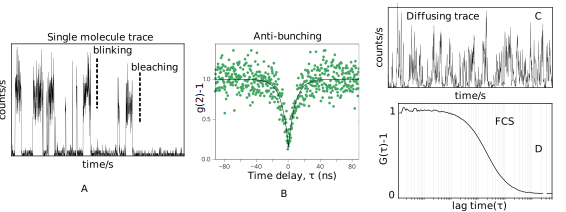
\includegraphics[width=\textwidth]{SM_characteristics}
	\caption{\textbf{Single-molecule characteristics.}
	(A) Time trace of a single molecule showing single-step switching (blinking) and bleaching.
	Notice the reappearance of the intensity after blinking but complete disappearance after bleaching.
	(B) Anti-bunching at zero delay time in the correlation shows the singleness of the emitter.\cite{chu2016a}
	(C) Time trace of diffusing molecules in a fluid with \SI{1}{\nM} fluorophores showing intensity bursts and the correlation amplitude ($G(\tau)-1={\sim}1$) indicating the presence of few molecules in the focus.}
	\label{fig:SM_characteristics}
\end{figure}

Fluorescence correlation spectroscopy (FCS) also considered as a single-molecule technique, measures the temporal correlation of fluctuating light intensities.\cite{magde1972thermodynamic,elson1974fluorescence,krichevsky2002fluorescence}
Conventional way to perform FCS is to collect signal from \textit{diffusing fluorescent} molecules in the diffraction limited focal volume and then compute the autocorrelation of the intensity trajectory.
The autocorrelation of the intensity signal is given as $G(\tau)=<I(t)I(t+\tau)>/<I(t)>^2$ where I is the intensity, $\tau$ the lag time and $<...>$ represents time averaging.
The correlation quantifies the probability the intensity at time $t$ is similar to the intensity at a later time $t+\tau$.
It provides information on the concentration and the time scale of the fluctuating observable.
By very nature, FCS technique requires the fluctuation of the number of diffusing fluorophores in the diffraction limited volume of \SI{1}{fL}, ideally one molecule in average.
Because of the diffraction limit ($\Delta{x}={\lambda}/2$), FCS is often limited to nanomolar and picomolar concentration of the analyte. 

Two of the important requirements to measure single molecules with high spatial and temporal resolution are (i) high fluorescence yield and (i) small excitation and detection volume.
In this thesis we push the limit of single-molecule detection to low quantum yield dyes and to a high concentration of fluorophore.

\section{TCSPC}
The fluorescence signals is normally recorded as intensity which is obtained by recording the voltage per unit time generated in a photo diode.
The advancement in sensitive detectors enabled the detection of the fundamental unit (quanta) of light, single photons.
Detailed information about a single molecule can be extracted when all the photons are registered in both space and time.
The time resolved technique used to record the information about photons is known as Time Correlated Single Photon Counting (TCSPC).\cite{oconnor2012timecorrelated,birch2002topics}
The technique require a pulsed laser with high repetition rate (\SI{\sim80}{\MHz}) and high time resolution (picoseconds).
TCSPC is suitable for low signal with less than one photons in average per laser pulse.
With each pulse of laser there is a probability of promotion of the molecule to the excited electronic state which depends on the excitation crossection, intensity of the laser and electronic state of the molecule.
Once excited the molecule may emit a photon whose probability depends on the radiative and nonradiative rate of the relaxation from its excited state.
The fluorescence lifetime can be given as:
\begin{equation}
	\tau = \frac{1}{\Gamma_{r} + \Gamma_{nr}}
\end{equation}
The arrival time of the emitted photon after laser pulse is called micro-time(t\_micro) and the absolute arrival time from the start of the measurement called macro-time(t\_macro).
\begin{figure}
	\centering
	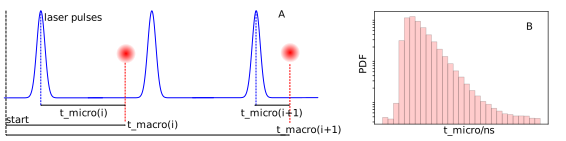
\includegraphics[width=\textwidth]{tcspc_sch}
	\caption{\textbf{TCSPC.} (A) The scheme for time resolve experiment showing the laser pulses as blue curve and subsequently detected photons as the red dots.
	The arrival time of emitted photons after the laser pulse is known as micro-time and the arrival time after the start of measurement is called macro-time.
	(B) The histogram of the micro-times gives the life time of the fluorophores.}
	\label{fig:tcspc_sch}
\end{figure}
The advantages of TCSPC measurements can be summarized as following:
\begin{itemize}
	\item \textbf{Binning free.} As each photon is recorded with its arrival time, TCSPC is binning free unlike the intensity measurements.
	From the photon arrival time, intensity traces with any binning time can be reproduced after the measurement.
	Dynamics of molecules on any time scale ranging from nanoseconds to seconds can be extracted and the time scale is only limited by resolution of the detector, the laser and total recording time.
	Fluorescence correlation spectroscopy (FCS) utilizes the leverages provided by TCSPC and gives dynamics on many orders of time scale in a single autocorrelation curve.
	\item \textbf{Lifetime.} Arrival times of photons (t\_micro) follow a Poisson distribution and the average fluorescence lifetime can be obtained by fitting the histogram of micro-time (Figure \ref{fig:tcspc_sch}B).
	Lifetime can not only give the intrinsic decay rate of the excited fluorophore, it also carries informations of the immediate sounding with which it interacts.
	Other applications of lifetime measurements are fluorescence resonance energy transfer (FRET), fluorescence lifetime imaging.\cite{selvin2000the,lakowicz1992fluorescence} 
	\item \textbf{Micro-Macro linking.} As each photon is stamped with micro and macro times, correlations can be extracted between the lifetime and dynamics of the macromolecules.
	Multiple fluorophores in a systems can be distinguished on the basis fluorescence lifetime.
\end{itemize}
In this thesis, almost every fluorescence measurement was  done with both micro and macro time stampings.
In Chapter-2, both micro and macro times are used to distinguish the shorter lifetime photons from the longer lifetime photons to correlation in FCS experiment.
Chapter-3 utilizes the inter-photon times (t\_macro(i+1) - t\_macro(i+1)) to extract information that can be mis-represented by the binning methods.
In chapter-4, the potential of TCSPC is tested to answer whether an enzyme is dynamically heterogeneous or monotonic. 
%
\section{Optical Nano-antennas for single molecules}
Single-molecule technique is limited to high quantum yield (\SI{>10}{\percent}) fluorophores or diluted number (\SI{\sim1}{\nM}) of molecules.
A large fraction of absorbing molecules including biomolecules and metal complexes show weak fluorescence with very low quantum yield (\SI{<1}{\percent}).
Additional auto-fluorescence in physiological environment often reduces the signal to noise ratio.
In addition, a majority of physiological reactions involving proteins and enzymes require milli to micro molar concentrations to perform usual activities.\cite{craighead2006future,punj2013gold,fabrizio2016roadmap,punj2014thesis}
Such physiology at micromolar concentrations can't be studied by the conventional microscopes.
Nano-plasmonics offer promising solution that can tackles both the concentration-limit by light-confinement and poor yield of dyes by enhancing their emission rates.

Optical nano-antennae are similar to the radio antennas at the macro scale.
Antennas are used to control and manipulate electromagnetic (EM) waves in the sub-wavelength scale.
Currents from a transmitter can be coupled to an antenna and radiated as EM wave to the far-field while on the other end EM waves in the far-field can be coupled to the antenna and send it to the receiver (Figure \ref{fig:nano_antenna}A,B).
Marconi used tens of meter antenna to control kilometer waves. 
The antennas can be scaled down to nanoscale to control nanometer waves which include the optical frequencies.
However the optical frequencies approach the frequency of the free electron on metals surface exciting their resonant frequencies called \textit{surface plasmon resonance (SPR)}.
Because of the plasmon excitation, they provide strong near-field enhancement and thus leading to confinement of EM waves to local hotshots.\cite{bath8624,schuller2010plasmonics,ozbay2006plasmonics,maier2005plasmonics,hess2012active}
In addition to SPR effect, the local electric field is also enhanced by the lightening rod effect which is a result of the high charge density at the curvatures or edges of the antennas.
Compared to $\lambda/2$ diffraction limit of light, plasmonics can confine light down to ${<}\lambda/10$.
\begin{figure}
	\centering
	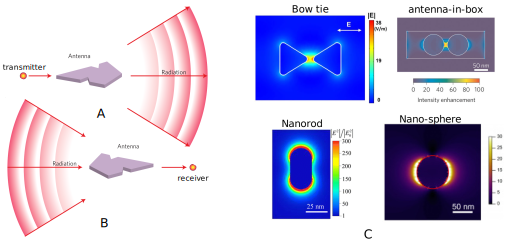
\includegraphics[width=\textwidth]{nano_antenna}
	\caption{\textbf{Optical nano-antenna.} Antenna coupled to the transmitter (A) and receiver (B) and the direction of energy flow is shown with the direction of the arrows.
	Free propagating light waves getting converted to localized energy and localized energy being radiated to the far-field.
	(C) Examples of nano antennas with their enhanced electric field.
	The color scales are indication of the electric field ($|E|$) or intensity ($|E|^2$) indicated close to the nano-structures.}
	\label{fig:nano_antenna}
\end{figure}
The fluorescence of an emitter placed in the near-field of a nano-antenna will be enhanced (i) by the high field and (ii) by acceleration decay rate.
Because of the high light intensity in the near-field, the fluorophore will be pumped harder which is known as excitation enhancement.
The transition probability of an emitter governed by the Fermi's Golden rule depends on the local density of states (LDOS) in addition to the transition matrix element between the two states.
Nano-antennas significantly modify the LDOS by enhancing the radiative rates of the emitter leading to increase in the quantum yield which is known as emission enhancement.
Close to the metal surface, additional non-radiative channels lead to quenching of fluorescence via losses.
Thus the resultant enhancement depends upon the emitter's position, orientation with respect to the antenna and overlap of its emission spectra with the resonance of the antenna.\cite{anger2006enhancement,khatua2014resonant}

The strength of the field enhancement and the field volume depends on the complexity of the nanostructure as shown in Figure \ref{fig:nano_antenna}C.
The goodness of an antenna is judged by the large field enhancement factor and smaller mode volume.
Bow tie antenna and antenna-in-box provides high field enhancement and small near-field volume but requires tedious and expensive lithographic expertise.\cite{novotny2011antennas,regmi2017thesis}
Gold nano-sphere is the simplest and cheapest form of nano-antenna but it gives low field enhancement and large near-field volume.\cite{punj2013gold}
Gold nanorods lies somewhere in the middle giving comparable field enhancement though with larger field-volume. For this thesis, gold nanorod remains the choice as a nano-antenna because:
\begin{itemize}
	\item Field enhancement is comparable to the best antennas available.
	\item The plasmon resonance can be tuned from green to far-infrared simply by changing the aspect ratio of the rod.\cite{link1999simulation}
	The width of the plasmon can be controlled as well by changing the volume of the rod.
	Narrow surface plasmon resonances is helpful for selective enhancement of emitters while broad resonance can be used to enhance broader spectrum of dye.\cite{yuan2013thousandfold,khatua2014resonant}
	\item Gold nanorods can be cheaply mass produced by colloidal synthesis methods with very smooth crystalline surface.\cite{nikoobakht2003preparation,perezjuste2005gold}
	\item Accessibility. As nanorods are small and colloidal in nature, they can be easily inserted into living cells.
	In fact, because of their luminescent nature, they are already being used in living cells or tissues for imaging.
	\item Selective reactivity. Gold is inert and harmless for the living organisms unlike other metals like silver.
	It has high affinity towards thiols opening the possibility of chemical functionalizations.
\end{itemize}
%
\section{Proteins at work are  proteins in motion}
Proteins and enzymes are the machinery inside living cells that perform both mechanical work and energy maintenance.
Often the proteins or enzymes are pictured by their static structures in crystallography or average structure of a large ensemble of conformations.
The functions of protein are governed by their dynamical motions.
A multidimensional energy landscape and different kinetic barriers govern the complex coordinated motion a protein requires.
A fourth dimension, time has been added to investigate their activity giving unprecedented insights to their physical properties.
Enzymes perform chemical reactions by binding with the substrate and minimizing the energy required for the product formation.
Spectroscopic studies done in the 80's and recent nuclear magnetic resonance (NMR) investigations show the amplitude and duration of structural fluctuation involved in the function of enzyme catalysis and protein function.
Movements are predicted in the time scale ranging from picoseconds corresponding to atomic movements to milliseconds involving movement of bigger domains.\cite{henzler-wildman2007dynamic,frauenfelder1991the}
The time scale of transitions rely on the energy barrier which are represented as energy landscape in the reaction coordinate.
The concept of energy landscape was first introduced by Frauenfelder and co-workers\cite{frauenfelder1991the} to explain the observation of multiple energy barriers and non-exponential kinetics in the rebinding of carbon monoxide and oxygen to myoglobin.
They connected the myoglobin function to the energy barriers and the existence of conformational sub-states.
Since then other studies by NMR and single-molecule technique have advanced our knowledge about the details of protein energy landscape.

\begin{SCfigure}[0.9][ht] %this figure will be at the right
    \centering
    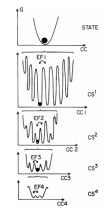
\includegraphics[width=0.4\textwidth]{energy_landscape}
    \caption{\textbf{Hierarchical arrangement of the conformational substates.} The energy landscape of protein showing hierarchical protein dynamics and energy barriers. The state represents the energy minima in one state the enzymatic reaction (one for reactant-state and one for product-state). Each state is composed of several substaes. Depending on the temperature upto four tiers can been found in the hierarchy.}
    \label{fig:energy_landscape}
\end{SCfigure}

An energy landscape is defined as a map of all possible atomic positions in a molecule and their corresponding energy levels typically Gibbs free energy.
A much more complex three dimensional energy landscape is typically represented in a two dimensional conformational co-ordinate (cc) system.
The hyper surface of energy landscape consists of number of valleys and in reality has a continuous and smooth distribution.
Each minima corresponding to the initial and final state of a reaction is called a ``state'' while each maxima is known as a ``transition state''.
Each state can assume a very large number of conformational substates and can be categorized into different tiers of energy(Figure \ref{fig:energy_landscape}).
The transition times directly relates to the energy barriers, the transitions in the tier-4 ($CS^4$) occurs in a faster time scale than in the tier-0($CS^0$).
The motions in protein can be categorized mainly into two types- equilibrium fluctuations (EF) and  functionally important motions (FIMs).\cite{ansari1985protein}
EFs involve motions among the substates and result in the equilibrium thermodyanmic properties like entropy and internal energy. 
The examples of EF include bond vibration, methyl rotation, loop motion and side chain rotaions.
However, FIMs are the non-equilibrium process between the states and involve structural changes in the larger domains of the protein.
If the initial and final states are closer in structure, they can be assumed to have similar substates. 
Larger changes in the structure during FIMs may relax the protein to different set of substates. This relaxation to a state with different substates lead to non-exponential distribution in their rates .

In this thesis, we will investigate the rate of complex formation between an electron transfer protein and their redox partners. We will relate their variation (heterogeneity) in rates to the changes in their structures.

\section{Azurin: An Electron Transfer Protein}
Electron transfer via oxidation and reduction control vital cellular processes like respiration, redox homeostasis, photosynthesis to name a few.
Proteins with a metal co-factor play a crucial role in carrying out such electron transfer.
Among the metalloproteins, Copper proteins are found in abundant carrying out activities like oxygen transport (hemocyanin), respiration (cytochrom-c oxidase) and metal homeostasis (ceruloplasmin) and electron transfer.
Because of their electron transport properties, metalloproteins are promising candidate for biosensors and biomolecular electronic devices.

Azurin is a copper(Type 1, T1) containing protein involved in electron transfer in cells.\cite{dennison2005investigating,kolczak2006handbook}
The Copper is buried in the northern side of azurin (MW=\SI{14}{\kilo\dalton}) being surrounded by a coordination sphere composed of two histidines, a cysteine and methionine\ref{fig:azurin_structure}.
The copper atom in azurin can posses either of the two oxidation states: Cu(II) and Cu(I).
Cu(II) azurin has a blue color due to the absorption at \SIrange{595}{630}{\nm} arising from $\pi - \pi^*$ transition in the molecular orbital scheme of azurin.\cite{dooley1981spectroscopic,schmauder2005sensitive}
In contrast, Cu(I) azurin is colorless as it has no absorption band in the red(Figure \ref{fig:flurox_azurin}.
Different spectroscopic characteristics of the two Cu-state can be used to measure kinetics of electron transfer of azurin.
The oxidation and reduction reactions via electron transfer is generally known as redox reaction.
The redox properties of azurin is determined by the Cu atom and the ligands surrounding Cu.
Azurin has a midpoint potential of \SI{60}{\mV}(vs Saturated Calomel Electrode, SCE) at pH 7.
Azurin is well characterized and is a reasonably stable protein at room temperature which makes it a suitable candidate for investigating fundamental properties of electron transfer reactions.
\begin{figure}
	\centering
	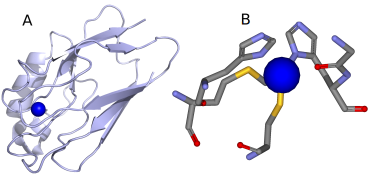
\includegraphics[width=\textwidth]{azurin_structure}
	\caption{\textbf{Azurin structure.} (A) Crystal structure (cartoon representation) of azurin from \textit{Pseudomonas aeruginosa}.\cite{adman1981structural}
	Copper atom is shown as a blue sphere.
	(B) Ligands around Copper atom: His117, His46, Cys112, Met121}
	\label{fig:azurin_structure}
\end{figure}

\section{Flurox Principle(FRET-redox)}
The absorption band at \SIrange{595}{630}{\nm} of azurin has been used to study electron transfer kinetics in ensemble.
To study electron transfer in single azurin molecule, a more sensitive background free fluorescence-technique in the red-infrared range can be used.
An external fluorescent marker is attached as azurin doesn't have intrinsic fluorescence in red.
If the emission spectrum matches (see Figure~\ref{fig:flurox_azurin}) with absorption of Cu(II) azurin, fluorescence will be quenched in oxidized state.
Whereas the fluorescence in Cu(I) will be bright due to the absence of quenching.
In another term, the oxidation state of the azurin can be read out simply by looking at the fluorescence of labeled azurin.
The principle to detect the oxidation state in metalloenzymes by looking at the fluorescence of an external marker is called FluoRox which was pioneered by Aartsma and co-workers.\cite{kuznetsova2008the,goldsmith2011redox,tabares2011fluorescence}
\begin{figure}
	\centering
	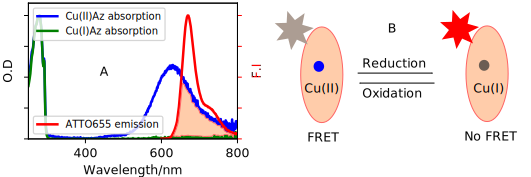
\includegraphics[width=\textwidth]{flurox_azurin}
	\caption{\textbf{Fluorox principle.} (A) Spectral overlap between the absorption of azurin and emission of ATTO655. Blue curve: absorption of Cu(II)azurin, green: absorption of Cu(I) azurin, red: emission of ATTO655.
	(B) Symbolic representation of the fluorescent state of azurin-ATTO655 in Cu(II)-state and Cu(I) state. In Cu(II) state, copper is shown as a blue sphere and the non-fluorescent ATTO655 is shown in gray. In Cu(I) state, copper is shown in green and the fluorescent ATTO655 is shown in red.}
	\label{fig:flurox_azurin}
\end{figure}
The efficiency of fluorescence quenching can be calculated similar to the energy transfer in ``fluorescence resonance energy transfer (FRET)'' which can be given as;
\begin{equation}
	E = \frac{R^6}{R_0^6 + r^6}	
\end{equation}
$R_0$ is the $F\ddot{o}ster$ radius at which the efficiency is \SI{50}{\percent} and $r$ is the distance between the Cu-atom and the dye.
$F\ddot{o}ster$ can be given as;
\begin{equation}
	R_0 = 0.211[\kappa^2n^{-4}Q_DJ(\lambda)]^{1/6}	
\end{equation}
where $\kappa^2$ is an orientation factor, n refractive index of the solvent, $Q_D$ quantum yield of the donor and $J(\lambda)$ spectral overlap between the absorption of azurin and emission of the dye.
The overlap between the emission of a dye ATTO655 and absorption of azurin can be visually seen in Figure~\ref{fig:flurox_azurin}A
ATTO655 attached at the Lys122 of azurin in buffer gives a quenching efficiency of \SI{90}{\percent}.
Such high quenching efficiency of Lys122 labeled azurin allows us to study electron transfer and their heterogeneity at single-molecule level(Chapter~5).

\section{This thesis}
The common theme of this is single molecule fluorescence. In the first part of the thesis, we try to improve signal from single molecules by plasmonic fluorescence enhancement, characterize the near field of the plasmonic structures from the statistics of enhanced signals. In the second part, we use the potential of single-molecule technique to enlighten our understanding about the conformational substates by looking at the electron transfer dynamics in azurin.

\begin{itemize}
	\item \textbf{Chapter 2.} Many physiological reactions like enzyme-substrate reactions occur in millimolar to micromolar concentration. Single-molecule studies doesn't allow to investigate at such a high concentration because of the diffraction-limited detection volume of few femtoliters. In this chapter, we use gold nanorod to perform fluorescence correlation spectroscopy (a branch of single-molecule technique) at physiologically relevant concentrations. The gold nanorod helped to confine light to smaller volumes and enhance the fluorescence. The fluorescent probe molecules (ATTO647N) were allowed to freely diffuse in a supported lipid bilayer. The zwitter ionic head groups on the lipid prevented any non-specific interaction with the substrate and the gold nanorod. Similar diffusion coefficients were observed in the far-field and near-field suggesting no influence of gold nanorod on the diffusing dyes. The diffusion time in the near-field and far-field allowed us to determine the near-field width of the gold nanorod. The fluorescence of the dye was enhanced maximum by a factor of five. The lower enhancement factor was attributed to the inaccessibility of the diffusing dyes to the hottest spot in the near field and the high quantum yield of the probe(\SI{70}{\percent}).
	The enhanced dyes had a shorter lifetime than the un-enhanced dye. By filtering out photons with longer lifetime, the correlation contrast was improved by more than two orders of magnitude. We also functionalized the bilayer with azurin-ATTO655 (biomolecule) and obtained similar improvement in the correlation contrast without any nonspecific interaction with the substrate.

	\item \textbf{Chapter 3.} More general way to characterize single-molecule time traces is to bin the trace and look for histogram and residence time of the transitions. The enhancement factor extracted from the time traces with gold nanorod were different for different binning time. We investigated the interphoton times to extract average enhancement factor and number of molecules in the near field. We performed numerical simulations and theoretical models to successfully extract the intensity distribution for slowly diffusing molecules in two dimensional bilayer. Number of molecules in the 2D Gaussian intensity profile were successfully predicted. We are continuing our investigation for the enhanced fluorescence where the detected intensity profile is more complicated.
	
	\item \textbf{Chapter 4.} Fluorescence enhancement factor by a single plasmonic structure varies strongly  (upto three orders of magnitude) depending on the position and orientation of the fluorescent probe. Furthermore, fluorescence bleaching limits the number of single molecules to one per single nanorod (in single-molecule study). In this chapter we use transient binding by DNA to repeatedly and reproducibly study many single molecules on a single nanorod on the same spot on its tip. The longer persistence length of DNA helps to keep the dye at a fixed distance from the tip. We optimized the passivation of gold nanorod surface to control the average number of binding site down to one and to minimize fluctuation of intensity of enhanced fluorescence.

	\item \textbf{Chapter 5.} In this final chapter, we investigated electron transfer in redox active single azurins. The oxidation state of the Cu-azurin was read out by observing the brightness of the fluorophore. Switching of Copper oxidation state was studied at different redox potentials where the potential was controlled electrochemically by a potentiostat. The distribution of midpoint potential was characterized both spatially and dynamically (longer time traces). The rate of complex formation between azurin and its redox partners showed correlated variations in time. As the variations were observed in steady state conditions and on a passive functionalized glass surface, the heterogeneity was attributed to the different conformation (substates) of azurin.
\end{itemize}
% \references{chapters/c1_intro/intro}